%\newcommand{\eps}{\epsilon}
\newcommand{\Pmax}{p_\text{max}} 	
\newcommand{\Hint}{H_{int}}
\newcommand{\kbar}{\bar{k}}
\newcommand{\Delk}{\Delta}
\newcommand{\Sumk}{\Sigma}
\newcommand{\Qrot}{Q_{pq}(\tau_s)}
\newcommand{\shapecor}{\mathcal{S}}
\newcommand{\ampcor}{\mathcal{A}}
\newcommand{\totalcor}{\mathcal{E}}
\newcommand{\threeLs}{L_p(\kbar_1)L_q(\kbar_2)L_r(\kbar_3)}
\newcommand{\threePs}{P_p(\kbar_1)P_q(\kbar_2)P_r(\kbar_3)}
\newcommand{\threeQs}{Q_p(k_1)Q_q(k_2)Q_r(k_3)}
\newcommand{\Lbasic}{\mathcal{P}_0}
\newcommand{\Linvk}{\mathcal{P}_1}
\newcommand{\Lnsinv}{\mathcal{P}^{n_s}_1}
\newcommand{\Lnsboth}{\mathcal{P}^{n_s}_{01}}
\newcommand{\Linvksq}{\mathcal{P}_2}
\newcommand{\Lns}{\mathcal{P}^{n_s}_2}
\newcommand{\Fbasic}{\mathcal{F}_0}
\newcommand{\Finvk}{\mathcal{F}_1}
\newcommand{\Finvksq}{\mathcal{F}_2}
\newcommand{\quadpot}{V_{\phi^2}(\phi)}
%\newcommand{\threeqs}{q_p(\kbar_1)\,q_r(\kbar_2)\,q_s(\kbar_3)}
\newcommand{\threeqs}{q_p(k_1)\,q_r(k_2)\,q_s(k_3)}
\newcommand{\threeqstilde}{q_{\tilde{p}}(k_1)\,q_{\tilde{r}}(k_2)\,q_{\tilde{s}}(k_3)}
\newcommand{\kmin}{{k_\text{min}}}
\newcommand{\kmax}{{k_\text{max}}}
\newcommand{\fnl}{f_{NL}}
\newcommand{\fnllocal}{f^{local}_{NL}}
\newcommand{\fnlequil}{f^{equil}_{NL}}
\newcommand{\fnlortho}{f^{ortho}_{NL}}

\chapter{Introduction to cosmology}\label{chapter:intro_general}
\section{General introduction}\label{sec:general_intro}
%\subsection{The bispectrum}
    \subsection{Fundamentals}
    General relativity tells us how the expansion of the universe depends
    on its matter and energy content.
    In the context of a spatially homogeneous and isotropic universe
    (known as a FLRW universe)
    the Einstein equations become the Friedmann equations.


    We begin with a homogeneous and isotropic metric with $c=1$
    \begin{align}
        ds^2 = a(t)^2 ds_3^2 - dt^2
    \end{align}
    where $a(t)$ will have the interpretation as the scale factor
    which describes the evolution of the universe.
    The components of the universe enter the equations through
    their stress-energy tensor, which we approximate as that of
    a perfect fluid
    \begin{align}
        T_{ab} = (\rho+P)U_aU_b+Pg_{ab}.
    \end{align}
    The quantity $w=\frac{P}{\rho}$ is constant,
    and takes the values $0$, $1/3$ and $-1$ for matter, radiation
    and dark energy respectively.
    The Einstein equation
    \begin{align}
        G_{\mu\nu} = 8\pi G T_{\mu\nu}
    \end{align}
    then gives us that
    for a flat universe with $\Lambda=0$
    \begin{align}
        H^2 &= \frac{8\pi G \rho}{3},\\
        \frac{\ddot{a}}{a} &= -\frac{4\pi G}{3}\left(\rho+3P\right),
    \end{align}
    where $H=\frac{\dot{a}}{a}$, and $\rho$ and $P$ are respectively the sum of the
    energy densities and of the pressure densities of the
    components of the universe.

    Given the equations of state and the densities of the different
    components of the universe, one can then calculate the time dependence of the
    scale factor $a(t)$. From this, one can understand how perturbations evolve, and understand
    how photons are redshifted as they freestream through the universe.


    Photons travel on geodesics. The geodesic equation that we use to determine
    their evolution is
    \begin{align}
        \frac{dP^a}{d\lambda}+\Gamma^a_{bc}P^bP^c=0.
    \end{align}
    Using the chain rule, this can be rewritten as
    \begin{align}
        P^{0}\frac{\partial P^a}{\partial t}+\Gamma^a_{bc}P^bP^c=0.
    \end{align}
    \textcolor{red}{REPHRASE ALL THIS}
    Writing the components of the photon's 4-momentum $P^a$
    as $(p, \mathbf{p})$ we get that
    \begin{align}
        p\propto \frac{1}{a}.
    \end{align}
    The interpretation of this result is that as the universe expands,
    the photon's energy decreases, and its wavelength increases.
    The geodesic equation encodes many other physical effects when applied
    to the evolution of perturbations around the homogeneous background,
    allowing us to understand how the statistics of the perturbations at the
    start of the $\lcdm$ evolution evolved into the perturbations we see today.


    We can rewrite the Friedmann equation as
    \begin{align}
        H^2 = H_0^2\left(\frac{\Omega_{r,0}}{a^4}+\frac{\Omega_{m,0}}{a^3}+\Omega_{\Lambda}\right)
    \end{align}
    where we define the fractional density
    \begin{align}
        \Omega_{X} = \frac{\rho_X}{\rho_{crit,0}}
    \end{align}
    for $X$ being radiation, matter and dark energy, using $\rho_{crit,0}$, the critical density for which the universe is flat.
    Let us take the future of the universe as an example, where $a$ is sufficiently large that $\Omega_{\Lambda}$
    is the dominant contribution to the expansion.
    Then
    \begin{align}
        H^2 &= H_0^2\Omega_{\Lambda}\\
        \implies \dot{a} &= \pm H_0\sqrt{\Omega_{\Lambda}}a
    \end{align}
    from which the initial conditions pick out the exponentially expanding solution,\\
    ${a(t)=a_0e^{H_0\sqrt{\Omega_{\Lambda}}\left(t-t_0\right)}}$. Using the Friedmann equation
    for sufficiently far in the future we can rewrite this as
    \begin{align}
        a(t)=a_0e^{H\left(t-t_0\right)}.
    \end{align}
    Then, using $ad\tau=dt$, we find that ${\tau(t)=(Ha_0)^{-1}\left(1-e^{-H(t-t_0)}\right)+\tau_0}$
    where as usual a $0$ subscript denotes a quantity evaluated today.
    This is the behaviour we would also like in the very universe, as we will see.

    \begin{table}[h!]
    \begin{center}
        \begin{tabular}{ c c c }
            Epoch & $a(t)$ & $a(\tau)$ \\ 
            \toprule
            Radiation & $t^{\frac{1}{2}}$ & $\tau$ \\
            Matter & $t^{\frac{2}{3}}$ & $\tau^2$ \\
            $\Lambda$ & $e^{Ht}$ & $-\frac{1}{\tau}$
        \end{tabular}\caption{
            How the scale factor, $a(t)$, evolves in the
            different epochs of the universe.
        }\label{lcdm_dep_table}
    \end{center}
    \end{table}


    Set-up the physical effects of transfer functions.


\begin{figure}[!pth]
\centering     %%% not \center
    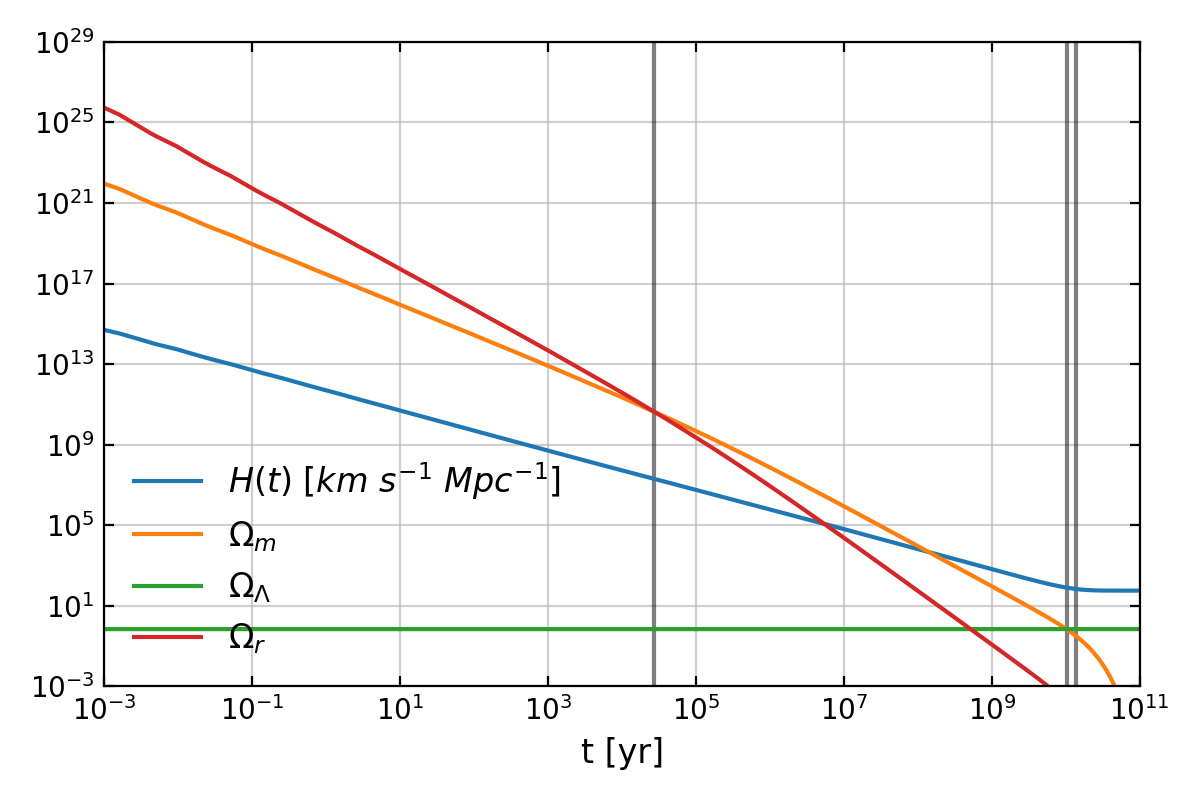
\includegraphics[width=.75\columnwidth]{plots/lcdm_components.png}
\caption{
    The evolution of the components of the universe up to the present, and slightly beyond.
    The vertical grey lines mark matter-radiation equality, matter-dark energy equality,
    and the present day, respectively. In the past, densities of matter and radiation were
    far higher, and the expansion of the universe ($H(t)$) was far stronger.
    In the future, as dark energy comes to dominate, $H(t)$ will become constant.
}\label{fig:lcdm_components}
\end{figure}
\begin{figure}[!pth]
\centering     %%% not \center
    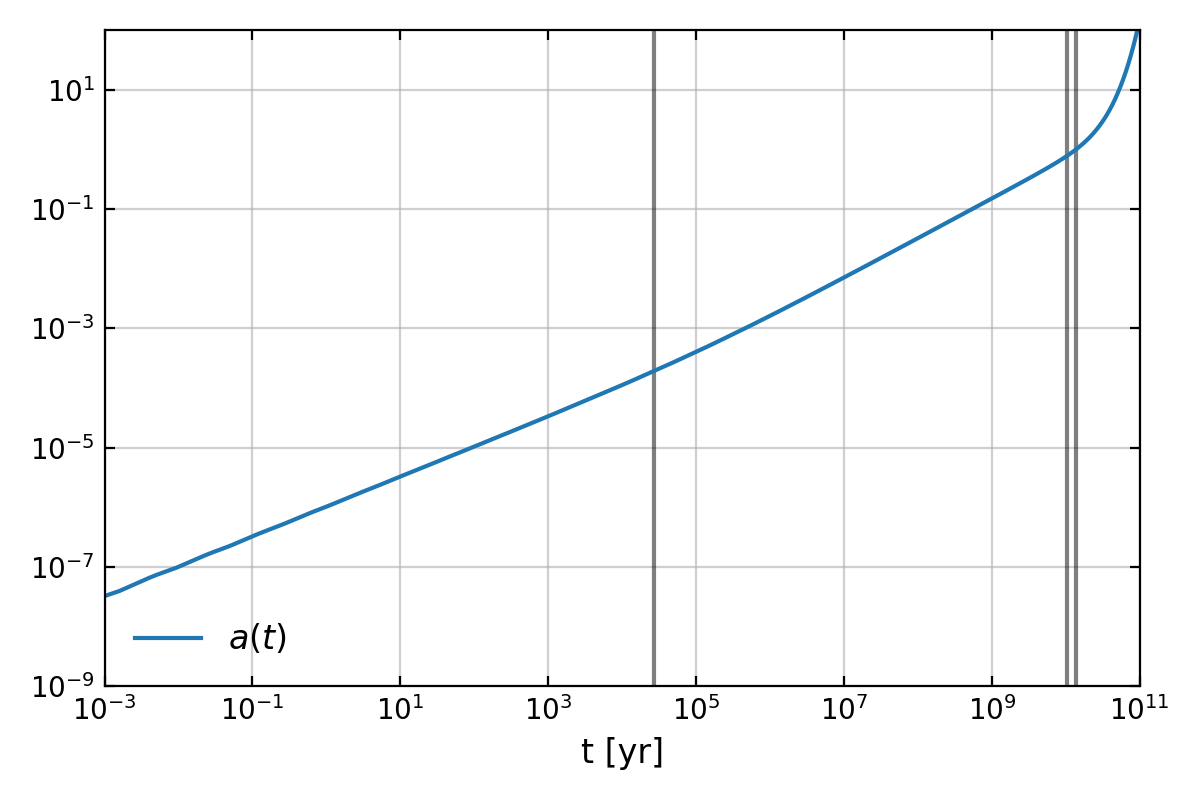
\includegraphics[width=.75\columnwidth]{plots/lcdm_a.png}
\caption{
    The evolution of the scale factor. For most of the $\lcdm$ history
    it evolves as some power of $t$, however as $\Lambda$ comes to dominate
    it will begin to grow exponentially.
}\label{fig:lcdm_a}
\end{figure}
\begin{figure}[!pth]
\centering     %%% not \center
    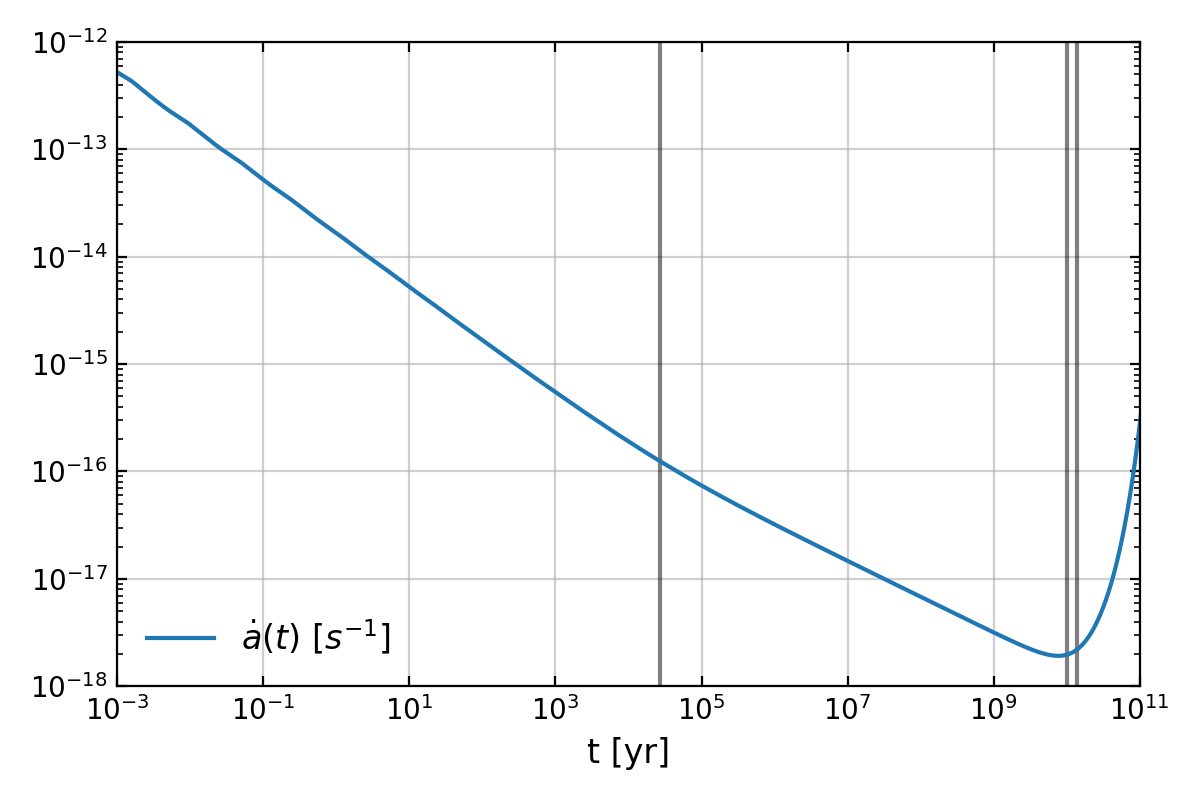
\includegraphics[width=.75\columnwidth]{plots/lcdm_adot.png}
\caption{
    During the radiation and matter dominated eras, the evolution of
    $a(t)$ as been slowing. However, as $\Lambda$ comes to dominate,
    the scale factor will begin to accelerate.
}\label{fig:lcdm_adot}
\end{figure}
\begin{figure}[!pth]
\centering     %%% not \center
    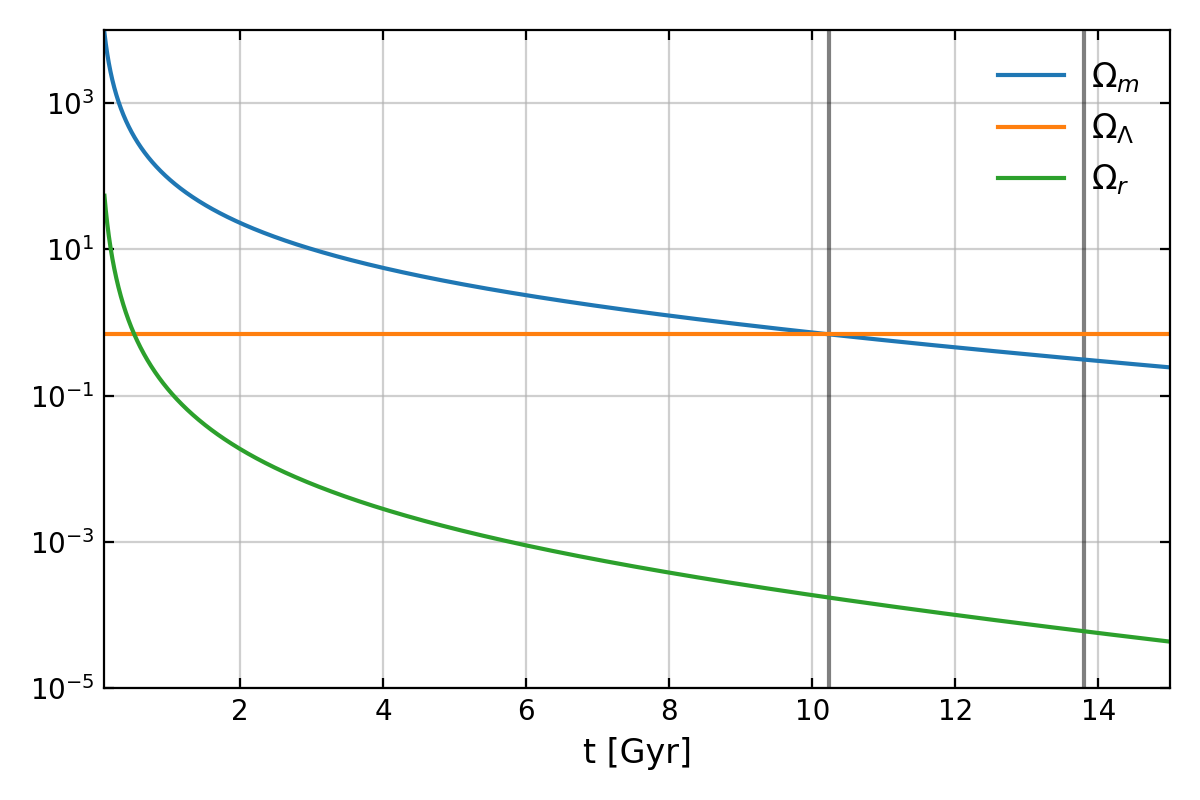
\includegraphics[width=.75\columnwidth]{plots/lcdm_components_linear.png}
\caption{
    The evolution of the components of the universe, zoomed in to more clearly
    show the matter-dark energy transition.
}\label{fig:lcdm_components_linear}
\end{figure}
\begin{figure}[!pth]
\centering     %%% not \center
    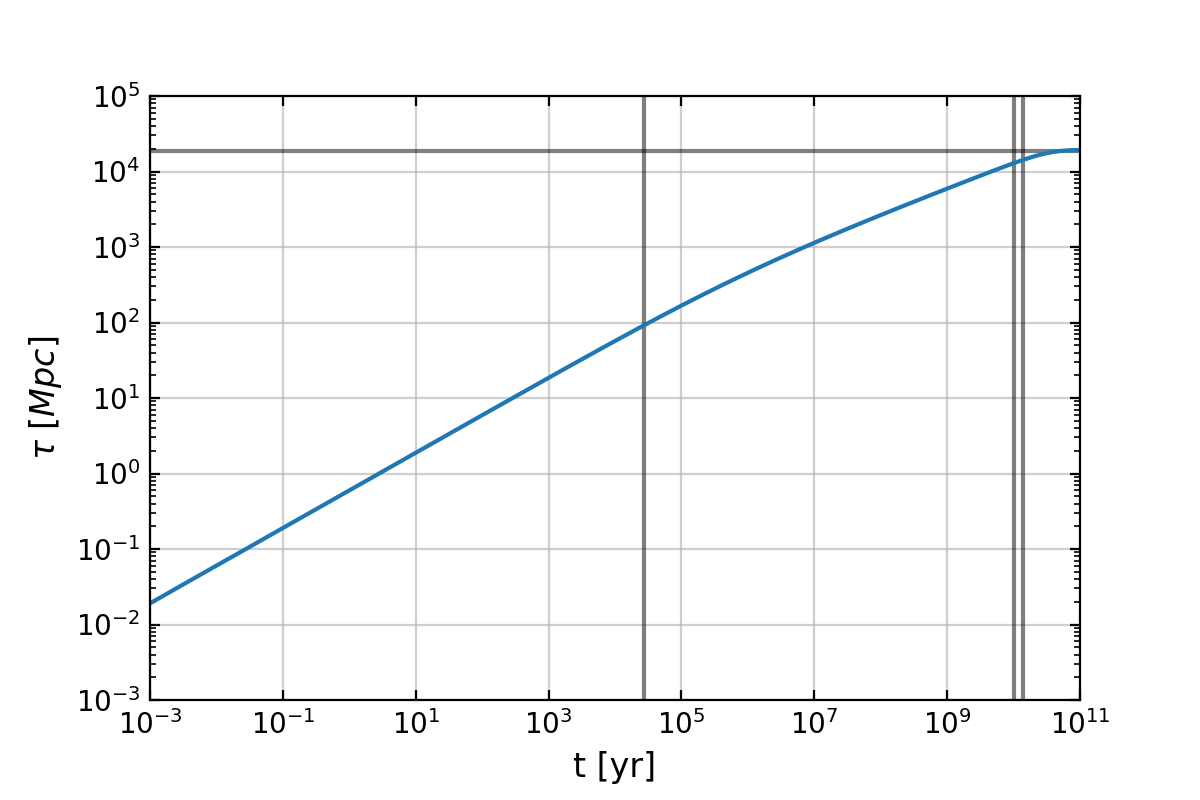
\includegraphics[width=.75\columnwidth]{plots/lcdm_tau.png}
\caption{
    The evolution of the conformal time $\tau$ since the $\lcdm$ singularity,
    if there is no inflation. Eventually $\tau$ will asymptote to a constant.
    \textcolor{red}{Physical interpretation at early and late times!!}
}\label{fig:lcdm_tau}
\end{figure}
\begin{figure}[!pth]
\centering     %%% not \center
    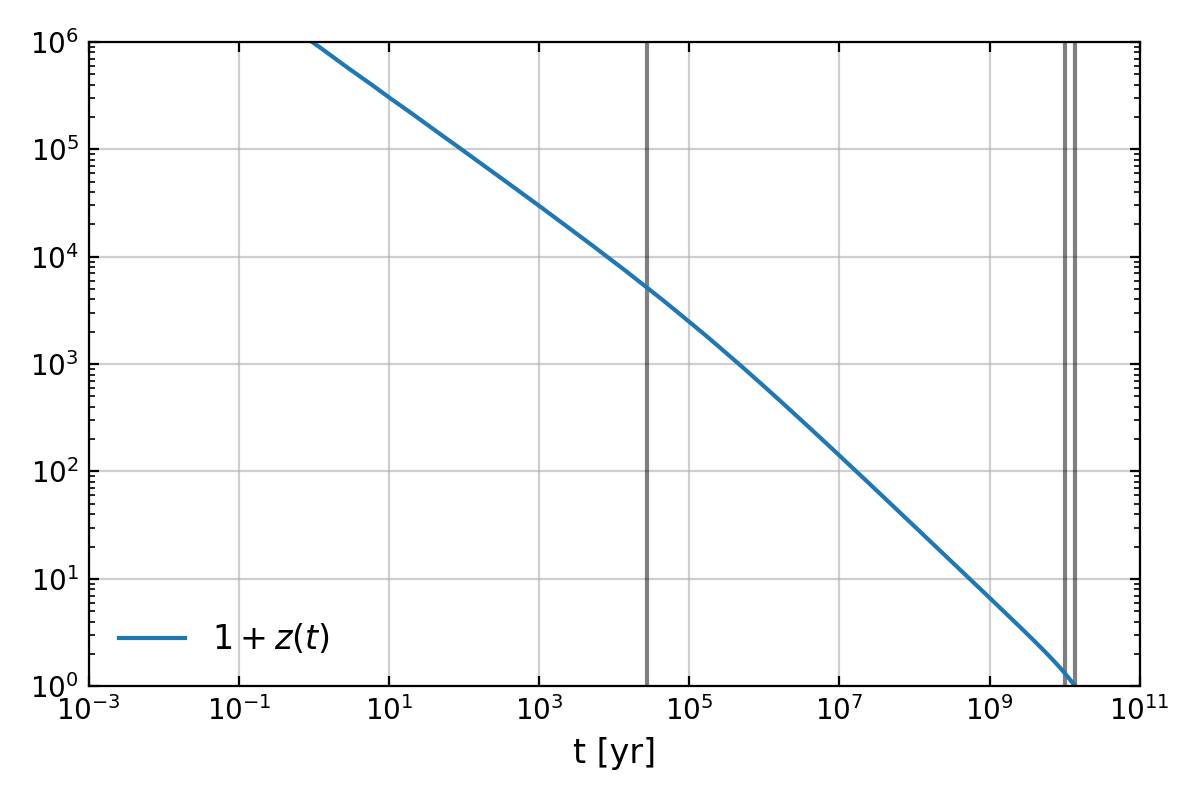
\includegraphics[width=.75\columnwidth]{plots/lcdm_z.png}
\caption{
    The correspondence between redshift $z$ and $t$.
    \textcolor{red}{Add temperature plot!!}
}\label{fig:lcdm_z}
\end{figure}

\newpage
    The history of the universe as a story of falling temperature.
\newpage
    \subsection{$\lcdm$}
    \textcolor{red}{Add references! Don't explain in detail, but do reference.}
    The $\lcdm$ model of the history of the universe assumes that at some point in the
    past, the components of the universe (all the different types of matter and radiation)
    were in thermal equilibrium with each other---that is, they were interacting with each other,
    and the interaction was sufficiently efficient that their temperatures matched
    and the net flow of thermal energy between them was zero.


    Recombination, what the $\cmb$ is.
    Plot of $a(t)$, $\tau(t)$ over all epochs.
    Path of a photon in $t-x$? Plot of $E(t)$?
\newpage
    Radiation is one of the major known components of the present universe, in the form of the
    photons in the cosmic microwave background, the $\cmb$. Another is matter, by which we mean \textit{dark} matter,
    which is invisible to our telescopes (which depend on electromagnetic radiation) but can be mapped by the
    effect of its gravity[ref]. Another component is what cosmologists refer to as baryonic matter, which is
    the protons, electrons, neutrons and all the other particles which make up the visible galaxies, stars
    and humans.
\newpage
    What is the evidence for $\lcdm$? Two main pieces of evidence are the relative abundances of
    primordial elements, and the baryon acoustic oscillations (BAOs).


    While it is thought that the heavier elements are made in incredibly energetic supernovae and
    neutron star collisions (such as lead[ref], or gold[ref]) the lightest elements are instead thought to have been forged in the
    very first minutes of the universes history. The $\lcdm$ model makes a detailed prediction as to the
    relative abundances of these elements, hydrogen, helium and lithium. It works well, but there is
    the ``lithium problem''.


    Baryon acoustic oscillations are the remnants of an epochal transition in the early universe.
    When the baryons decoupled from the radiation (due to the falling temperature) they were dropped,
    no longer supported by the photon pressure. They began to collapse back into the gravitational
    wells the dark matter had been forming. The imprint of this can be seen in the statistics
    of the positions of galaxies in the sky \textcolor{red}{Did I use the zooming out thing in
    BlueSci? Can I use it here??} [ref two-point], we will discuss two-point statistics in
    section \textcolor{red}{ref}.
\newpage
    Future work on $\lcdm$ includes the solution of the Hubble tension---how old is the universe really?
    All in all, it is incredible only a hundred years ago people were debating whether the universe had a beginning or not
    (and the ``great debate''---were there other galaxies?) to now, where the debate rages over the second and third significant
    figures.
\newpage
\section{Initial conditions for $\lcdm$}
    \subsection{Motivations for inflation}
    The $\lcdm$ model does not posit a ``Big Bang singularity'', though this is often
    how it is described in popular science communication. Instead, as we have discussed, it
    posits an early epoch in which the components that we have discussed are in thermal equilibrium,
    at an incredibly hot temperature of \textcolor{red}{number}. These components are distributed incredibly uniformly,
    with inhomogeneities of less than \textcolor{red}{number}. This simple scenario then evolves
    under gravitational collapse (and other interactions) and forms the universe we know.


    Is this story of $\lcdm$ enough to explain all the features of the
    universe that we observe? The answer is mostly less, given the correct initial conditions,
    the correct starting point. But then that begs the question of how those initial conditions
    were chosen out of the other possibilities one could imagine.
    Two clues that we have are known as the horizon problem, and the flatness problem.
    Roughly speaking, these problems are the statements that the universe is more homogeneous on
    large scales than we would expect, given the history of $\lcdm$. Why is the temperature on one
    part of the sky so close to the temperature on the other side of the sky? Why is the universe
    so flat?
\newpage
    Photons travelling on $45'$ lines on a $\tau-x$ plot. There not being enough time for opposite
    sides of the $\cmb$ to come into thermal equilibrium. But if you change the relation between
    $t$ and $\tau$ then you extend the plot, and you do make contact.
\newpage
    We desire a period of exponential expansion in the early universe to explain the
    scale-invariance of the initial perturbations.
    One simple way one could imagine driving this expansion is through a single
    scalar field. This scalar field would have
    \begin{align}
        \rho_\phi &= \frac{1}{2}\dot{\phi}^2+V(\phi)\\
        P_\phi &= \frac{1}{2}\dot{\phi}^2-V(\phi).
    \end{align}
    For successful inflation with a cosmological constant, we want $w=-1$,
    i.e.\ that $V(\phi)\gg\frac{1}{2}\dot{\phi}^2$. Since the kinetic term is required to
    be small, this is referred to as \textit{slow-roll} inflation.
    The Friedmann equations then become
    \begin{align}
        H^2 &\approx \frac{8\pi G V(\phi)}{3},\\
        \frac{\ddot{a}}{a} &= -\frac{4\pi G}{3}\left(-2V(\phi)\right),
    \end{align}
\newpage
    \subsection{Criteria for successful inflation}
    Sufficient e-folds, matching the statistics of the primordial perturbations.
\newpage
    Could talk briefly about alternatives? E.g.\ kinetic dominance.
\newpage
\section{Statistical observables}
    \subsection{Checking dice for fairness}
    The prediction of the fundamental quantum theory is a statistical one,
    i.e.\ a prediction of the distribution from which our observation will be drawn.
    As such, we need to talk in terms of estimators, estimating how likely it
    would be to see the sky we do, assuming some fundamental theory.


    Our result will be a constraint on an inflationary parameter, stated at e.g.\ $95\%$ confidence.
    For example, if we flipped one fair coin $100$ times, we would expect an even split of heads
    and tails. Should we be suspicious of the fairness of the coin if we instead get $60$ heads
    and $40$ tails? Or $80$ heads and $20$ tails? An event at least as extreme at a $60$-$40$ split
    will occur $3.5\%$ of the time. For a $80$-$20$ split however, the probability of an event that
    extreme is around one part in $10^{10}$, effectively impossible. This means that if we observed
    a trial where a coin came up heads in $80$ out of $100$ cases, we could suspect that out hypothesis
    of fairness was incorrect.
    One can calculate that, for a fair coin, $95\%$ of the time the events will fall within the
    range $[41,59]$. We call this the $95\%$ confidence interval.
    What we wish to do is the opposite, however. Instead of calculating using known probabilities,
    we wish to take a series of observations of some random variable and use these observations
    to estimate the probability distribution that they were drawn from. Given an infinite number
    of observations this task has a straightforward solution, simply plotting the normalised
    histogram of the results. However, in the context of cosmology we will only have a finite amount
    of information available to us, and thus a limit to how well we can ever measure the relevant
    probability distributions. This limitation is known as cosmic variance.



    We quantify this expected scatter around the mean using a quantity known as the standard deviation.
    The standard deviation of a random variable $X$ is the square root of the expected value of the
    squared deviation from the mean $\mu$,
    \begin{align}
        \sigma = \sqrt{E\left[{(X-\mu)}^2\right]}.
    \end{align}
    In our example above of flipping one coin $100$ times, the total number of heads has $\mu=50$
    and $\sigma=5$.

    
    We have only one universe that we can observe, only one draw from the probability distribution
    we are trying to probe. However, there is a lot of information in that one draw.
    \textcolor{red}{Motivate and explain this all better!} This is related to the concept
    of ergodicity. This is the statement that $\left<\cdot\right>$ as an expectation over ensembles
    at a fixed point is the same as the expectation over point for a fixed ensemble.
    This assumes homogeneity, stationarity, and that distant points are uncorrelated.
    In terms of our coin example, this is related to the statement that flipping one coin
    $100$ times should probe the probability distribution in the same way as flipping
    $100$ identical coins once each.
    %Ergodicity: ``In an ergodic scenario, the average outcome of the group is the same as the average outcome of the individual over time. An example of an ergodic systems would be the outcomes of a coin toss (heads/tails). If 100 people flip a coin once or 1 person flips a coin 100 times, you get the same outcome.'' from https://taylorpearson.me/ergodicity/
    % See also https://nms.kcl.ac.uk/eugene.lim/AdvCos/lecture2.pdf


    We can define the expectation value of a function of a discrete or
    continuous random variable $x$, or a functional $F$ of a field configuration $f(x)$, respectively as
    \begin{align}
        \left<f(x)\right> &= \sum_i x_i P(x_i)\label{expectation_value_discrete}\\
        \left<f(x)\right> &= \int dx~x \rho(x)\label{expectation_value_cont}\\
        \left<F\left[f(x)\right]\right> &= \int \mathcal{D}f~F\left[f(x)\right] P\left[f(x)\right]\label{expectation_value_field}
    \end{align}
    where the sum and integral over $x$ are over the values that $x$ can take,
    and the functional integral over $f$ is over all the field configurations
    that $f(x)$ can take.


    In our example of the $100$ coin flips, we used~\eqref{expectation_value_discrete}
    to calculate the mean and standard deviation. For a continuous variable,
    like the average height of a population or the average temperature in a given room,
    we would use~\eqref{expectation_value_cont}. In this thesis, we will be working with
    the expectation value of field configurations, so we will use~\eqref{expectation_value_field}.
    \textcolor{red}{Talk about quantum to classical transition!}
    \begin{align}
        \left<\hat{v}_{\bk},\hat{v}_{\bk'}\right>
                         &= \left<0|\hat{v}_{\bk},\hat{v}_{\bk'}|0\right>\\
                         &= |v_k|^2\left<0\left|\left[\hat{a}_\bk,\hat{a}_{-\bk}^{\dagger}\right]\right|0\right>\\
                         &= |v_k|^2\delta(\bk+\bk')\\
                         &= P_{v}(k)\delta(\bk+\bk')
    \end{align}


    \subsection{Power spectra}
    The power spectrum and other correlations
    are predicted by inflation. 
    Define n-point correlations, their Fourier transforms, talk about them as observables.
    

    A model of inflation will predict the statistical properties of the distribution of matter
    that forms the initial conditions for the $\lcdm$ evolution of our universe.
    From this, we can calculate the statistical properties of the $\cmb$ sky that we see.
    One such property is the two-point correlation of the temperature $\phi$
    at a point $x$ on the sky, $\left<\phi(x)\phi(x')\right>$. When there is a large
    angular separation between $x$ and $x'$ \textcolor{red}{talk about cosmic variance
    of different modes.}
\newpage
\section{Observational data}
    \subsection{\planck, Simons} 
    High-level descriptions.
    What fraction of the sky did they look at?
    Did they include polarisation?
    What was their angular resolution?
\newpage
    \subsection{Future missions}
    High-level descriptions.
    What fraction of the sky will they look at?
    Will they include polarisation?
    What will their angular resolution be?
\newpage
\section{Outline of thesis}
\textcolor{red}{Should some of this be moved to the end of chapter 2? Maybe a high-level outline here
and then a technical outline at the end of chapter 2.}
    \subsection{Goals}
    \begin{enumerate}
        \item Connecting inflation models directly to observations,
            through the bispectrum.
        \item Constraining the parameters of inflation models, not phenomenological templates and $f_{NL}$.
        \item To obtain the full shape information, not point samples or a limit.
        \item Efficient numerics gives access to more accurate, and in some cases new, feature shapes.
    \end{enumerate}
\newpage
    \subsection{Methods}
    \begin{enumerate}
        \item Building separability into the tree-level in-in formalism.
        \item The CMB calculation~\cite{Sohn_2021}: expensive, but need only be done once per primordial basis.
        \item So, we want a basis expansion that converges quickly for a broad range of inflation models.
        \item Convergence on the cube is different to the tetrapyd.
        \item Turns out to be much faster at primordial level than previous numerical methods
            (as it in a sense converges way faster, and as it enables us to use faster numerical methods than otherwise).
    \end{enumerate}
\newpage
    \subsection{Results}
    \begin{enumerate}
        \item First development/implementation of the formalism for calculating the expansion to high orders.
        \item We recognised and described the central issue of the cube vs tetra problem.
        \item Found a basis with broad descriptive power (and other less powerful basis sets).
        \item This allowed the first validation of these methods on features.
        \item Connect to CMB, get constraints on DBI $c_s$.
    \end{enumerate}

The thesis is organised as follows. In chapter~\ref{chapter:intro_bispectra} we present brief reviews
of the various parts of the pipeline that connects inflation scenarios to observations
through the bispectrum.
We review the usual paradigm of bispectrum estimation in the CMB,
and the motivation for separable bispectra. We review the in-in formalism,
for calculating the tree level bispectrum for a given model of inflation.
We review $P(X,\phi)$ models of inflation as an example, and
some of the usual approximate bispectrum templates
that we aim to bypass.
We will draw our validation scenarios from these models.
We discuss previous numerical codes for
calculating the primordial bispectrum $k$-configuration by $k$-configuration,
which contrasts our separable basis expansion.
We review the previous work in achieving separability through modal expansions
in~\cite{Funakoshi},
and we discuss methods of testing
numerical bispectrum results, defining our relative difference measurement.
In chapter~\ref{chapter:methods} we present our methods.
Since the paradigm we aim to present is only viable if we can find a basis
that can efficiently represent a wide variety of bispectra,
we begin with this distinct and separate, but nonetheless vital, discussion.
We discuss the effects of the
non-physical $k$-configurations on the convergence of our expansion on
the tetrapyd, and present an efficient basis.
Then, we recast the usual in-in calculation into an explicitly separable form,
in terms of an expansion in an arbitrary basis,
and detail our methods for carefully calculating the coefficients to high order.
In section~\ref{sec:validation} we validate our methods and implementation
on inflation scenarios with varied features from the literature,
and we finish with a discussion of future work in chapter~\ref{chapter:conclusion}.

